\documentclass[12pt]{article}
\usepackage{graphicx} % Required for inserting images
\usepackage{newtxtext} % This package sets Times New Roman as the main font
\usepackage{ragged2e} % This package is used to justify the text
\usepackage{setspace} % This package is used to set the line spacing
\usepackage[a4paper, left=3.0cm, top=3.0cm, bottom=2.0cm, right=2.0cm]{geometry} % This package is used to set the margins
\usepackage{lipsum} % This package is used to generate filler text
\usepackage{fancyhdr} % This package is used to customize the headers and footers
\usepackage{titlesec} % This package is used to customize titles
\usepackage[portuguese]{babel} % This package is used to translate the names of the document elements
\usepackage{hyperref} % This package is used to create hyperlinks in the document
\usepackage{indentfirst}
\setlength{\parindent}{1.25cm}  % This command sets the size of the indent
\usepackage{siunitx}
\sisetup{
  output-decimal-marker = {,},
  inter-unit-product = \ensuremath{{}\cdot{}},
  per-mode = symbol
}
\DeclareSIUnit{\real}{R\$}
\newcommand{\real}[1]{R\$#1}
\usepackage{float}
\usepackage{footnotehyper}
\usepackage{hyperref}
\hypersetup{
    colorlinks=true,
    linkcolor=black,
    filecolor=magenta,      
    urlcolor=cyan,
    pdfborder={0 0 0},
}
\usepackage[normalem]{ulem} % [normalem] prevents the package from changing \emph{} command
\makeatletter
\def\@pdfborder{0 0 0} % this line is needed to change the border color to white
\def\@pdfborderstyle{/S/U/W 1} % this line is to underline the links
\makeatother
\onehalfspacing

\begin{document}

\begin{titlepage}
    \centering
    \vspace*{1cm}
    \Large\textbf{INSPER – INSTITUTO DE ENSINO E PESQUISA}\\
    \Large ADMINISTRAÇÃO/ECONOMIA\\
    \vspace{1.5cm}
    \Large\textbf{INTUITO DO DOCUMENTO - "MATÉRIA"}\\
    \vspace{1.5cm}
    Prof. "Nome do Professor"\\
    Profa. Auxiliar "Nome do Monitor"\\
    \vfill
    \normalsize
    Aluno1, \href{mailto:aluno1@al.insper.edu.br}{aluno1@al.insper.edu.br}\\
    Aluno2, \href{mailto:aluno21@al.insper.edu.br}{aluno2@al.insper.edu.br}\\
    "Periodo e Turma"\\
    \begin{figure}[h]
    \centering
    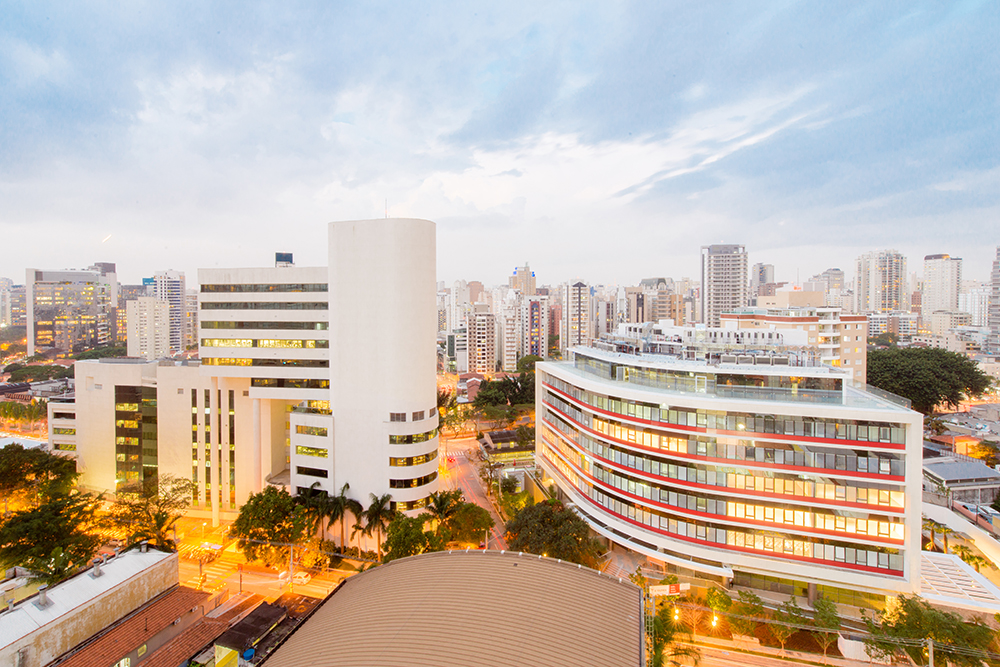
\includegraphics[width=0.5\textwidth]{campus-insper-22.jpg}
    \caption{Sua legenda aqui} 
    \label{fig:my_label}
    \end{figure}
    \vfill
    São Paulo\\
    Mês/Ano
\end{titlepage}

\newpage
\tableofcontents
\thispagestyle{empty} % This command removes the page number from the table of contents page
\newpage
\setcounter{page}{1} % This command sets the page number to start from this page
\justify
\onehalfspacing

\pagestyle{fancy}
\fancyhf{}
\rhead{\thepage}
\lfoot{Nota de rodapé}

\section{\textbf{Capítulo 1}}
\begin{table}[H]
\centering
\caption{Insira a legenda da tabela aqui}
\begin{tabular}{|c|c|c|c|c|}
\hline
\textbf{Coluna 1} & \textbf{Coluna 2} & \textbf{Coluna 3} & \textbf{Colunas ...} & \textbf{Coluna n} \\ \hline
Valor 1           & Valor 2           & Valor 3           & Valor ...    & Valor N1          \\ \hline
Valor 4           & Valor 5           & Valor 6           & Valor ...    & Valor N2          \\ \hline
\end{tabular}
\label{tab:my_label}

\footnotesize{Fonte: Elaborado pelos autores.}
\end{table}

\subsection{\textbf{Seção 1}}
\subsubsection{\textbf{SubSeção 1}}
\newpage

\section{\textbf{Capítulo 2}}
\subsection{\textbf{Seção 1}}
\subsubsection{\textbf{SubSeção 1}}
\newpage


\section{\textbf{Capítulo 3}}
\subsection{\textbf{Seção 1}}
\subsubsection{\textbf{SubSeção 1}}
\newpage

\section{\textbf{Capítulo 4}}
\subsection{\textbf{Seção 1}}
\subsubsection{\textbf{SubSeção 1}}

\newpage
\begin{thebibliography}{9}
\section{\textbf{Bibliografia Consultada}}
Bibliografia Consultada no formato ABNT
\end{thebibliography}

\newpage
\appendix
\section{Apêndice}
Este é o Apêndice 

\end{document}
